\documentclass{beamer}
\usepackage{listings}
\usetheme[pageofpages=of,% String used between the current page and the
                         % total page count.
          bullet=circle,% Use circles instead of squares for bullets.
          titleline=true,% Show a line below the frame title.
          alternativetitlepage=true,% Use the fancy title page.
          titlepagelogo=circl-logo.pdf,% Logo for the first page.
%          watermark=watermark-polito,% Watermark used in every page.
%          watermarkheight=100px,% Height of the watermark.
%          watermarkheightmult=4,% The watermark image is 4 times bigger
                                % than watermarkheight.
          ]{Torino}

\usepackage[utf8]{inputenc}
\usepackage{tikz}
\usepackage{transparent}

\author{Alexandre Dulaunoy CIRCL - \emph{TLP:WHITE}}
\title{Blackhole Networks}
\subtitle{a source of intelligence to support investigations}
\institute{Team CIRCL}
\date{\today}

\begin{document}

\begin{frame}[t,plain]
\titlepage
\end{frame}

\begin{frame}
        \frametitle{Enforce information sharing overview}
        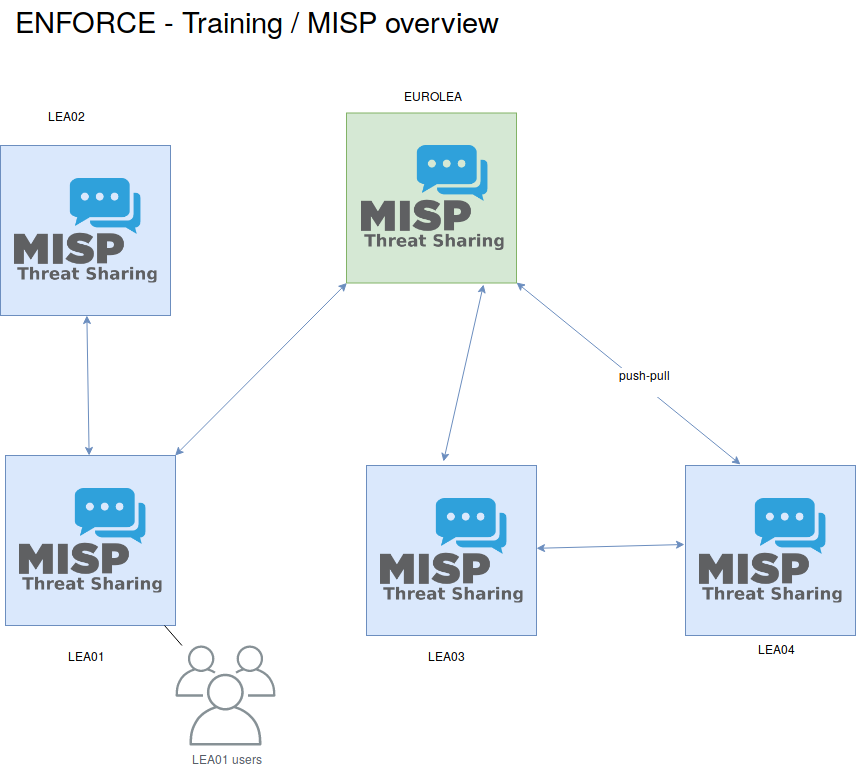
\includegraphics[scale=0.28]{enforce-misp.png}
\end{frame}

\begin{frame}
\frametitle{Workshop details}
\begin{itemize}
        \item 48 pcaps (2 days) are distributed (TLP:GREEN) from two blackhole networks (193.168.81.0/27 - 185.194.92.0/22)
        \item During the workshop, {\bf each team can analyse the network capture without restriction} (any tools can be used) and {\bf interesting discoveries can be shared} during the session (e.g. via MISP)
        \item Content of the network captures are unknown to CIRCL, the goal is to have an interactive session to share findings and techniques
\end{itemize}
\end{frame}

\begin{frame}
\frametitle{Motivation and background}
\begin{itemize}
    \item IP darkspace or black hole is
    \begin{itemize}
        \item {\bf Routable non-used address space} of an ISP (Internet Service Provider),
        \item incoming traffic is unidirectional
        \item and {\bf unsolicited}.
    \end{itemize}
    \item Is there any traffic in those darkspaces?
    \item If yes, what and why does it arrive there?
    \begin{itemize}
            \item And {\bf on purpose} or {\bf by mischance}?
    \end{itemize}
    \item What's the security impact?
    \item What are the security recommendations? How can we use the information to improve traffic analysis?
    \item Terminology: Honeypot versus darkspace
\end{itemize}
\end{frame}

\begin{frame}
\frametitle{The infinite value of crap}
        {\center \it \Huge 4 years in the life of a printer\\}
        \begin{flushright}
        from a series of packets hitting our darkspace
        \end{flushright}
\end{frame}

\begin{frame}[fragile]
\frametitle{Printer sending syslog to the IP darkspace}

\begin{verbatim}
2014-03-12 18:00:42
   SYSLOG lpr.error printer: offline
     or intervention needed
2014-03-23 21:51:24.985290
   SYSLOG lpr.error printer: paper out
   ...
2014-08-06 19:14:57.248337
   SYSLOG lpr.error printer: paper jam
\end{verbatim}
\end{frame}



\begin{frame}
\frametitle{4 years in the life of a printer}
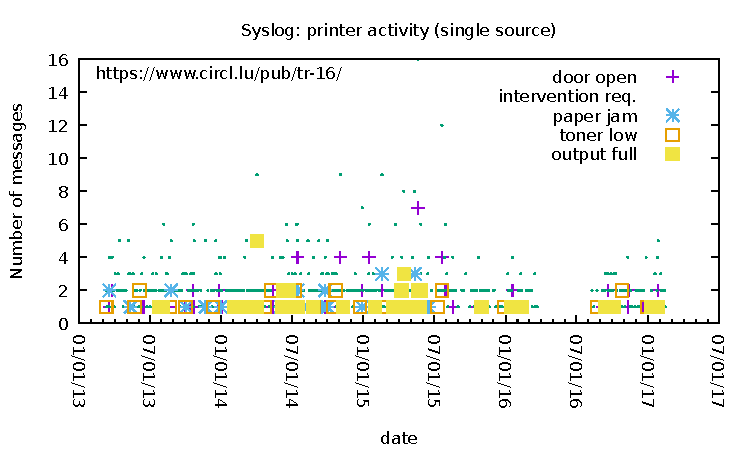
\includegraphics[scale=0.90]{printer.pdf}
\end{frame}

\begin{frame}
\frametitle{Business days based on the printer activity}
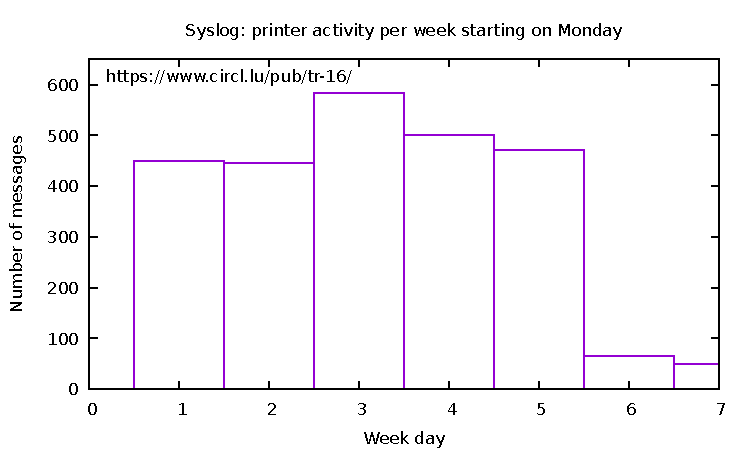
\includegraphics[scale=0.90]{printerweek.pdf}
\end{frame}

\begin{frame}
\frametitle{Printer activity and business hours}
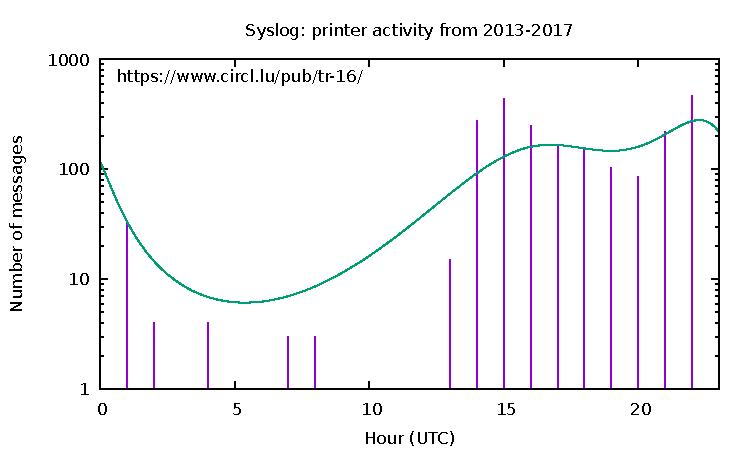
\includegraphics[scale=0.90]{printerhours.pdf}
\end{frame}

\begin{frame}
\frametitle{Where is the printer?}
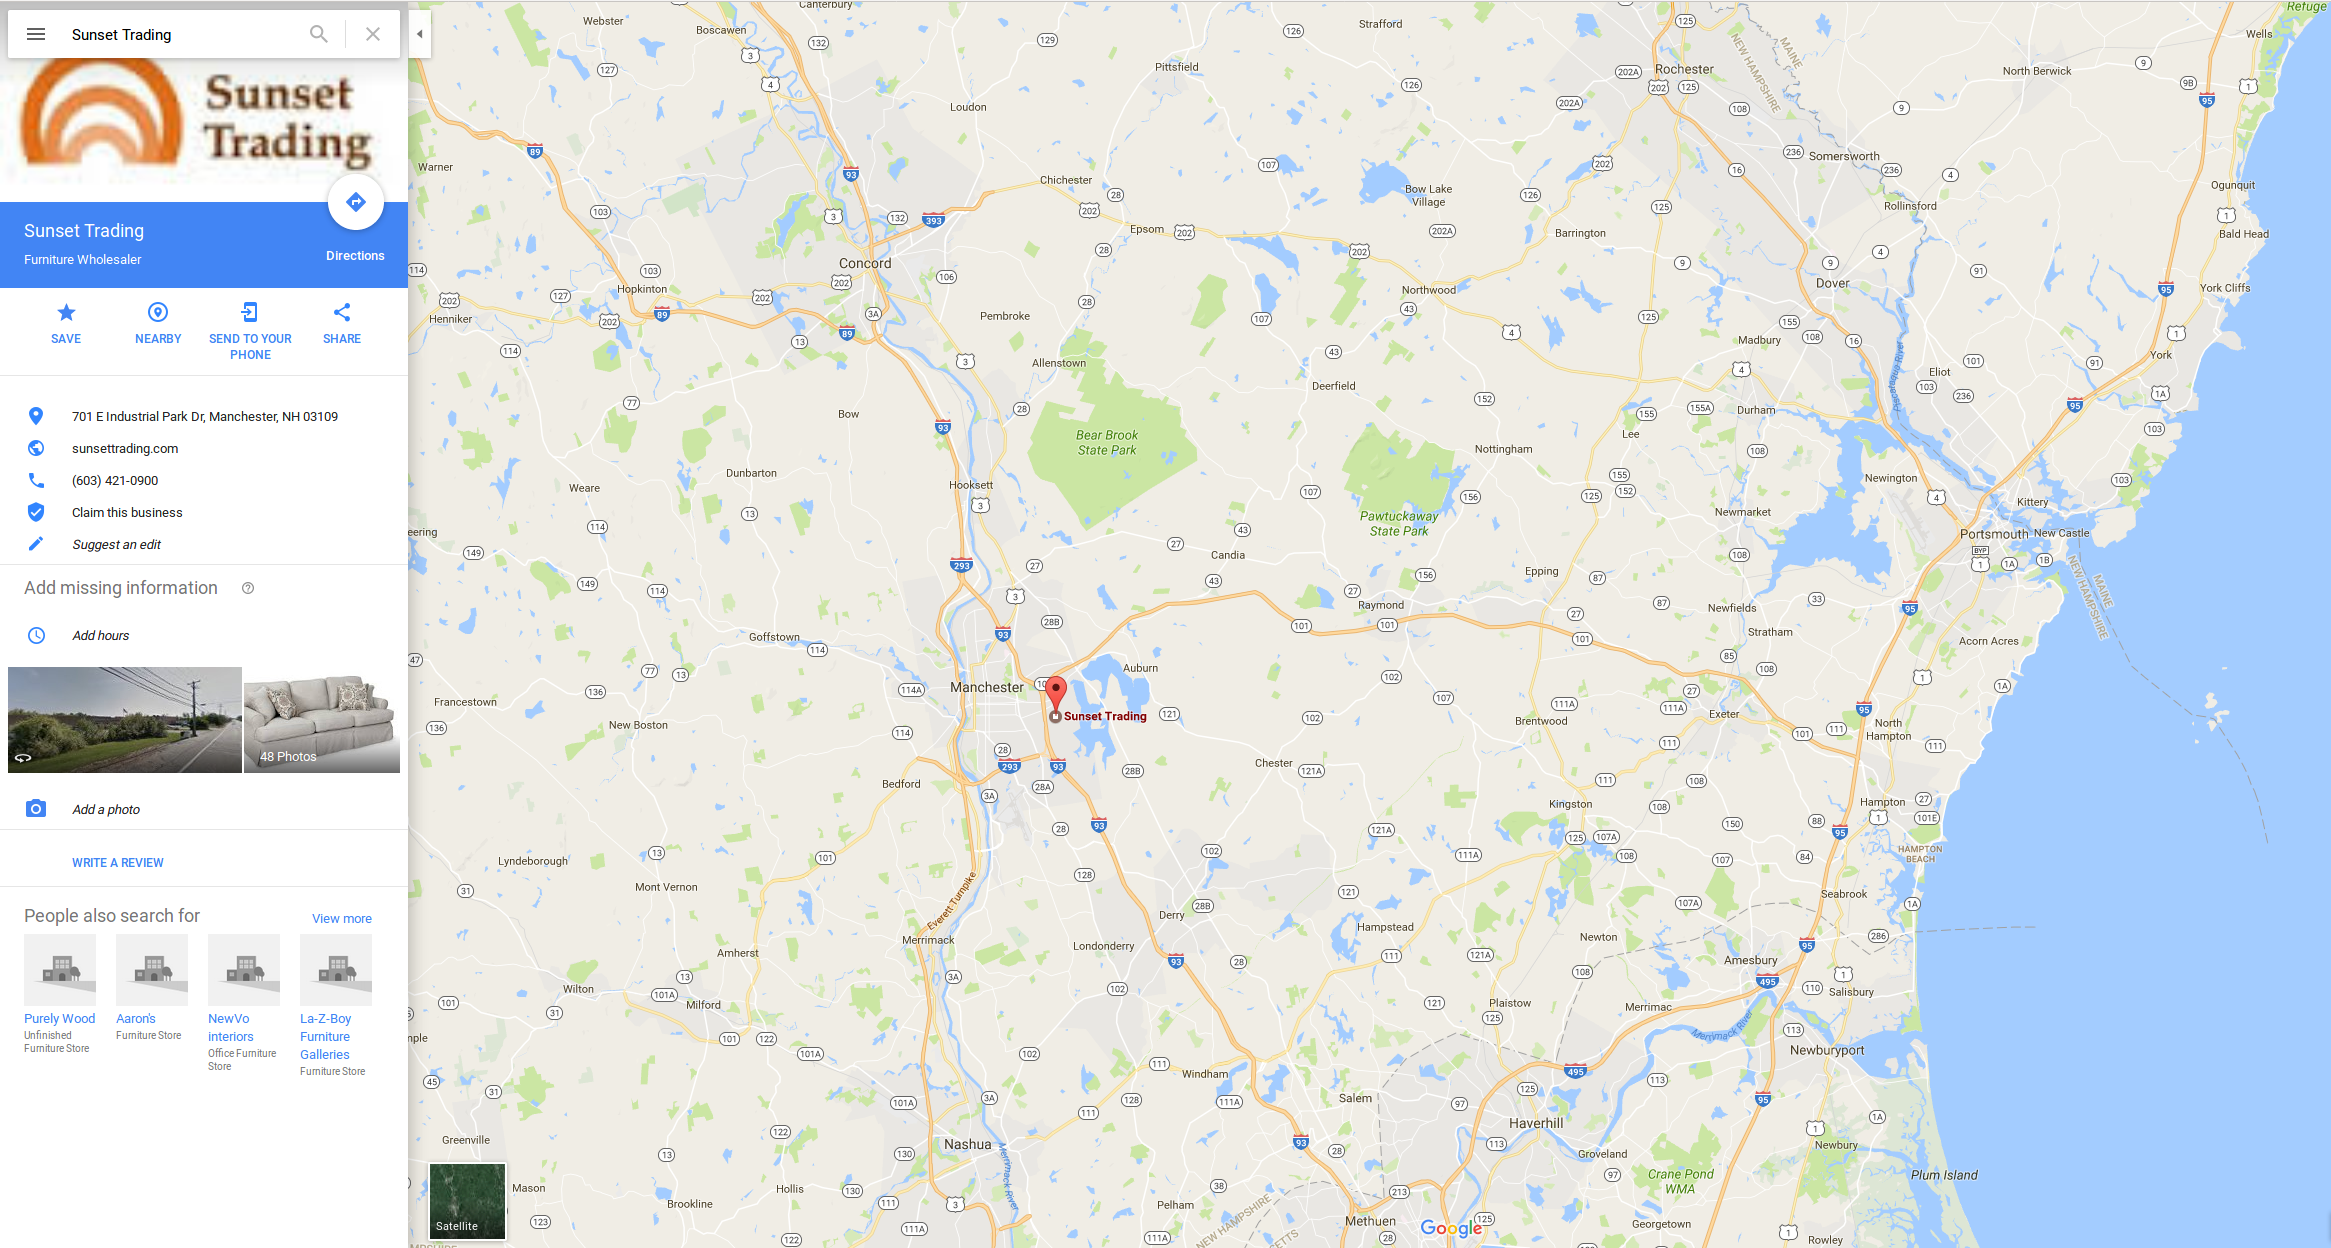
\includegraphics[scale=0.20]{sunset.png}
\end{frame}

\begin{frame}
\frametitle{Origin of traffic in the black hole}
\begin{itemize}
    \item Attackers (and researchers) scan networks to find vulnerable systems (e.g. SSH brute-force)
    \item Backscatter traffic (e.g. from spoofed DoS)
    \item Self-replicating code using network as a vector (e.g. conficker, residual worms)
    \item Badly configured devices especially embedded devices (e.g. printers, server, routers)
    \begin{itemize}
        \item $\rightarrow$ \textbf{Our IP darkspace is especially suited for spelling errors from the RFC1918 (private networks) address space}
    \end{itemize}
\end{itemize}
\end{frame}

\begin{frame}
\frametitle{Why is there traffic}
\framesubtitle{Typing/Spelling errors with RFC1918 networks}
    \begin{itemize}
        \item While typing an IP address, different error categories might emerge:
\end{itemize}
\begin{tabular}{lll}
Hit wrong key & 19\textbf{2}.x.z.y $\rightarrow$ & 19\textbf{3}.x.y.z\\
&172.x.y.z & 1\textbf{5}2.x.y.z\\
Omission of number & 1\textbf{9}2.x.y.z $\rightarrow$ &12.x.y.z\\
Doubling of keys &10.a.b.c $\rightarrow$ & 10\textbf{0}.a.b.c\\
\end{tabular}

\end{frame}



\begin{frame}
\frametitle{Research activities related to spelling errors}
\framesubtitle{Spelling errors apply to text but also network configuration}
\begin{itemize}
    \item 34\% omissions of 1 character
    \begin{itemize}
        \item Example: Network $\to$ Netork
    \end{itemize}
    \item 23\% of all errors happen on 3rd position of a word
    \begin{itemize}
        \item Example: Text $\to$ Test)
    \end{itemize}
        \item 94\% spellings errors are single errors in word
        \begin{itemize}
            \item And do not reappear
        \end{itemize}
\end{itemize}

\begin{block}{References}
    \begin{itemize}
        \item Pollock J. J. and Zamora A., Collection and characterization of spelling errors in scientific  and scholarly text. J. Amer. Soc. Inf. Sci. 34, 1, 51 58, 1983.
        \item Kukich K., Techniques for automatically correcting words in text. ACM Comput. Surv. 24, 4, 377-439, 1992.
    \end{itemize}
\end{block}
\end{frame}

\begin{frame}
\frametitle{DDoS and blackhole}
        {\center \it \Huge backscatter traffic\\}
        \begin{flushright}
        why DDoS victims are not always silent
        \end{flushright}
\end{frame}

\begin{frame}
        \frametitle{DDoS overview}
        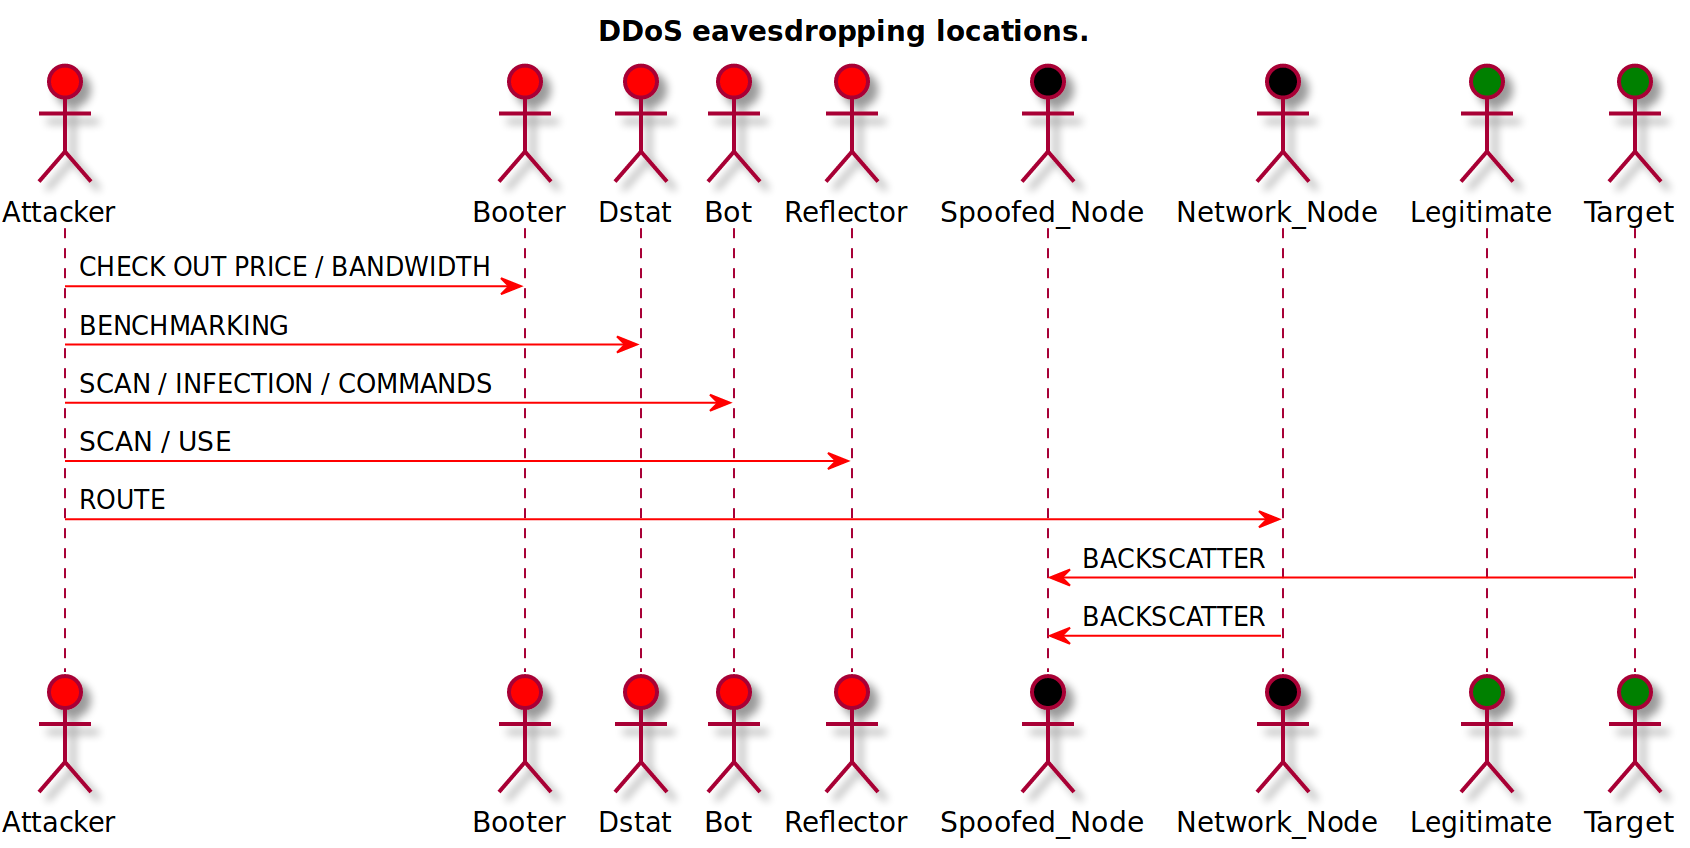
\includegraphics[scale=0.2]{ddos-overview.png}
\end{frame}

\begin{frame}
\frametitle{Observing SYN floods attacks in backscatter traffic}
Attack description

    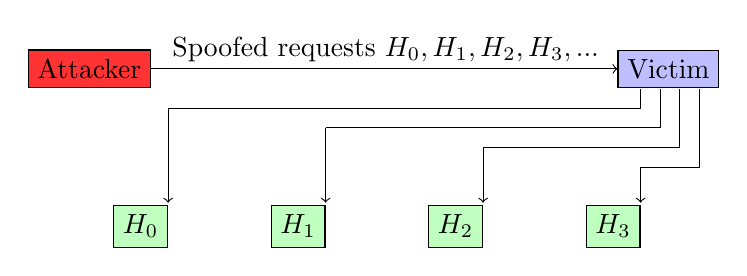
\begin{tikzpicture}{scale=0.4}
    \node[rectangle,draw,fill=red!80] (a) at (0,0) {Attacker};
    \node[anchor=west] at (0.93,0.25) {Spoofed requests $H_{0},H_{1},H_{2},H_{3},...$};
    \node [rectangle,draw,fill=blue!25,anchor=east] at (8,0) (v) {Victim};
    \draw [->](a) --(v);

    \foreach \x in {0,1,2,3} {
        \node [rectangle,draw,fill=green!25,anchor=east] at (\x*2+1,-2) {$H_{\x}$};
        %Horizontal lines
        \draw (\x*2+1, -\x*0.25-0.5)--(7.0+\x*.25,-\x*0.25-0.5);
        %Links to the victim
        \draw (7.0+\x*.25,-\x*0.25-0.5) -- (7.0+\x*.25,-0.25);
        %Links to hosts
        \draw[->] (\x*2+1, -\x*0.25-0.5)--(\x*2+1,-1.70);
    }
    \end{tikzpicture}


\begin{center}
    \begin{tabular}{|l|}
        \hline
        Connections\\
        \hline
        $H_{0}$\\
        \hline
        $H_{1}$\\
        \hline
        $H_{2}$\\
        \hline
        $H_{3}$\\
        \hline
    \end{tabular}
\end{center}

\begin{center}
Fill up state connection state table of the victim
\end{center}

\end{frame}

\begin{frame}
\frametitle{How does backscatter look like?}
\lstset{%                                                                       
  backgroundcolor=\color{gray!25},                                              
  basicstyle=\ttfamily,                                                         
  breaklines=true,                                                              
  columns=fullflexible                                                          
} 
\begin{lstlisting}
2017-09-16 10:02:22.807286 IP x.45.177.71.80 > x.x.105.167.39468: Flags [.], ack 1562196897, win 16384, length 0
2017-09-16 10:02:27.514922 IP x.45.177.71.80 > x.x.121.213.62562: Flags [.], ack 14588990, win 16384, length 0
2017-09-16 10:02:28.024516 IP x.45.177.71.80 > x.x.100.72.30395: Flags [.], ack 24579479, win 16384, length 0
2017-09-16 10:02:30.356876 IP x.45.177.71.80 > x.x.65.254.17754: Flags [.], ack 318490736, win 16384, length 0
\end{lstlisting}

\begin{center}
    \alert{What are the typical characteristics?}
\end{center}
\end{frame}
\begin{frame}
    \frametitle{Is it DDoS backscatter traffic?}
    \begin{block}{Problem}
        \begin{itemize}
            \item Distinguish between compromised infrastructure and backscatter
            \item Look at TCP flags $\to$ filter out single SYN flags
            \item Focus on ACK, SYN/ACK, RST...
            \item Do not limit to SYN/ACK or ACK $\to$ ECE (ECN Echo)/CWR\footnote{\url{https://tools.ietf.org/html/rfc3168}}
        \end{itemize}
    \end{block}
    \lstset{%
    backgroundcolor=\color{gray!25},
    basicstyle=\ttfamily,
    breaklines=true,
    columns=fullflexible
}

\begin{lstlisting}
tshark -n -r  capture-20170916110006.cap.gz -T fields -e frame.time_epoch  -e ip.src -e tcp.flags
1505552542.807286000 x.45.177.71 0x00000010
1505552547.514922000 x.45.177.71 0x00000010
\end{lstlisting}

\end{frame}


\begin{frame}
\frametitle{What can be derived from backscatter traffic?}
\begin{itemize}
    \item {\bf External point of view} on ongoing denial of service attacks
    \item Confirm if there is a DDoS attack
    \item Recover time line of attacked targets
    \item Review targeted services (DNS, webserver, $\dots$)
    \item Infrastructure changes (e.g. change of routing)
    \item Assess the state of an infrastructure under denial of service attack
    \begin{itemize}
        \item Detect failure/addition of intermediate network equipments, firewalls, proxy servers etc
        \item Detect DDoS mitigation devices
    \end{itemize}
    \item Tools, Techniques and Tactics\footnote{\url{https://www.misp-project.org/taxonomies.html\#\_ddos\_2}} used by the attackers
\end{itemize}
\end{frame}

\begin{frame}
\frametitle{Getting DDoS attack information or validation}
\framesubtitle{Example nationalcrimeagency.gov.uk}
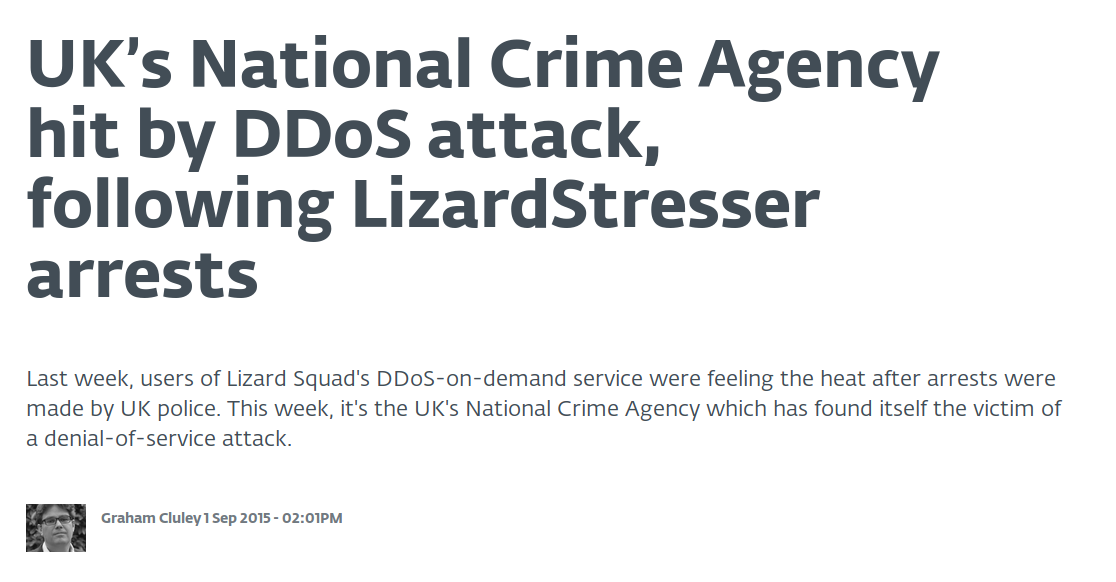
\includegraphics[scale=0.3]{article.png}
\end{frame}

\begin{frame}[fragile]
\frametitle{Getting additional information}
\framesubtitle{Example nationalcrimeagency.gov.uk}

        \begin{itemize}
                \item Gather potential IP addresses (via DNS or Passive DNS)
                \item Check all records type (A, AAAA, MX, CNAME)
        \end{itemize}
\begin{verbatim}
nslookup nationalcrimeagency.gov.uk

Server:         127.0.0.53
Address:        127.0.0.53#53

Non-authoritative answer:
Name:   nationalcrimeagency.gov.uk
Address: 194.61.183.46
\end{verbatim}
\end{frame}


\begin{frame}[fragile]
\frametitle{Getting additional information on DDoS attacks}
\framesubtitle{Example nationalcrimeagency.gov.uk}
\small
\begin{verbatim}

find files/2015/08/28/ -type f | parallel -j 7 '
    tcpdump -n -r {1} "host 194.61.183.46"'

17:10:06.857475 IP 194.61.183.46.80 > x.x.109.194.17293
   Flags [S.], seq 1635851834, ack 1801912321, win 0, length 0
17:10:14.869661 IP 194.61.183.46.80 > x.x.109.73.58142:
   Flags [S.EW], seq 1066513712, ack 4190371841, win 0, length 0
17:10:14.881036 IP 194.61.183.46.80 > x.x.111.106.49231:
   Flags [S.EW], seq 1531124927, ack 252116993, win 0, length 0
17:10:15.186684 IP 194.61.183.46.80 > x.x.102.45.62535:
   Flags [S.EW], seq 486934691, ack 536346625, win 0, length 0
17:10:18.946674 IP 194.61.183.46.80 > x.x.67.46.62399:
   Flags [S.EW], seq 234597292, ack 4069785601, win 0, length 0
\end{verbatim}
\end{frame}

\begin{frame}
    \frametitle{Dealing with DDoS claims}
    \framesubtitle{Screenshots from the attacker are valuable information}
    \begin{center}
        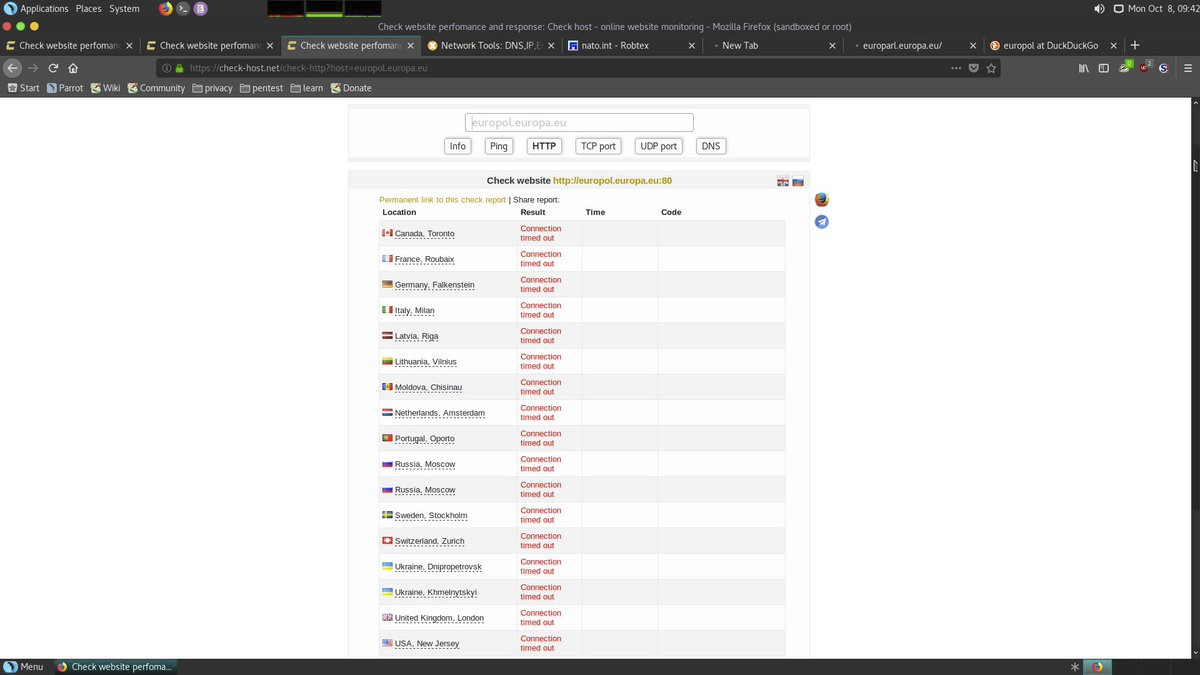
\includegraphics[scale=0.25]{screenshot.png}
    \end{center}
\end{frame}

\begin{frame}
    \frametitle{Dealing with DDoS claims}
    \framesubtitle{Screenshots from the potential attacker are valuable information}
    \begin{itemize}
        \item If some operational security is done
        \begin{itemize}
            \item Hide displayed hints (i.e. user name, IP address, country)
        \end{itemize}
        \item Local time
        \item Used operating system
        \item Used browser
        \item Used browser plugins
        \item Bookmarks
        \item Open other tabs
        \item Configured search engines
        \item Some cases images contains meta data such as exif
        \item {\bf Validating the claims} against DDoS backscatter
    \end{itemize}
\end{frame}

\begin{frame}
        \frametitle{DDoS backscatter limitation or drawbacks}
        \begin{itemize}
                \item Visibility limited by the spoofed networks from the DDoS attackers
                \item The size of the network telescope
                \item The state of the network infrastructure from the victims (e.g. how long the infrastructure is active)
                \item If the conditions are there, {\bf only a subset of the returned packets will be received}
        \end{itemize}
\end{frame}


\begin{frame}
\frametitle{How to write a Gartner market survey?}
        {\center \it \Huge What are the most common antivirus software?\\}
        \begin{flushright}
        by using the DNS queries hitting your darkspace
        \end{flushright}
\end{frame}

\begin{frame}[fragile]
\frametitle{Sample subset of DNS queries towards antivirus vendors domains}
\lstset{ %
%language=Python,                % choose the language of the code
basicstyle=\footnotesize,       % the size of the fonts that are used for the code
numbers=left,                   % where to put the line-numbers
numberstyle=\footnotesize\color{cyan},      % the size of the fonts that are used for the line-numbers
stepnumber=1,                   % the step between two line-numbers. If it is 1 each line will be numbered
numbersep=5pt,                  % how far the line-numbers are from the code
backgroundcolor=\color{white},  % choose the background color. You must add \usepackage{color}
showspaces=false,               % show spaces adding particular underscores
showstringspaces=false,         % underline spaces within strings
showtabs=false,                 % show tabs within strings adding particular underscores
rulecolor=\color{red},
frame=single,           % adds a frame around the code
tabsize=2,          % sets default tabsize to 2 spaces
captionpos=b,           % sets the caption-position to bottom
breaklines=true,        % sets automatic line breaking
breakatwhitespace=false,    % sets if automatic breaks should only happen at whitespace
escapeinside={\%*}{*)}          % if you want to add a comment within your code
}
\begin{lstlisting}
0.0.0.16a8.20ae.2f4a.400.7d.igkhab8lsrnzhj726ngu8gbsev.avqs.mcafee.com A INET 127.161.0.128
0.0.0.16a8.20ae.2f4a.400.7d.sdszgsg5a6j516p9nui9jfz5mj.avqs.mcafee.com A INET 127.161.0.128
40.ucp-ntfy.kaspersky-labs.com
46.ucp-ntfy.kaspersky-labs.com
6.ucp-ntfy.kaspersky-labs.com
dnl-06.geo.kaspersky.com.<COMPANYNAME>.local
shasta-mr-clean.symantec.com
shasta-mrs.symantec.com
shasta-nco-stats.symantec.com
\end{lstlisting}
\end{frame}

\begin{frame}
        \frametitle{Scripting your statistics for antivirus installations}
        \begin{itemize}
                \item Extract {\bf a list of words} from VirusTotal (antivirus products supported)
                \item Match the DNS queries with extracted words (e.g. be careful with fake antivirus)
                \item {\bf Filter per source IP address} (or aggregated subnets) to limit the result per organisation
                \item Plot the number of hits per aggregated words using in a single antivirus product name
        \end{itemize}
\end{frame}

\begin{frame}
\frametitle{A/V Statistics from Misconfigured Resolvers}
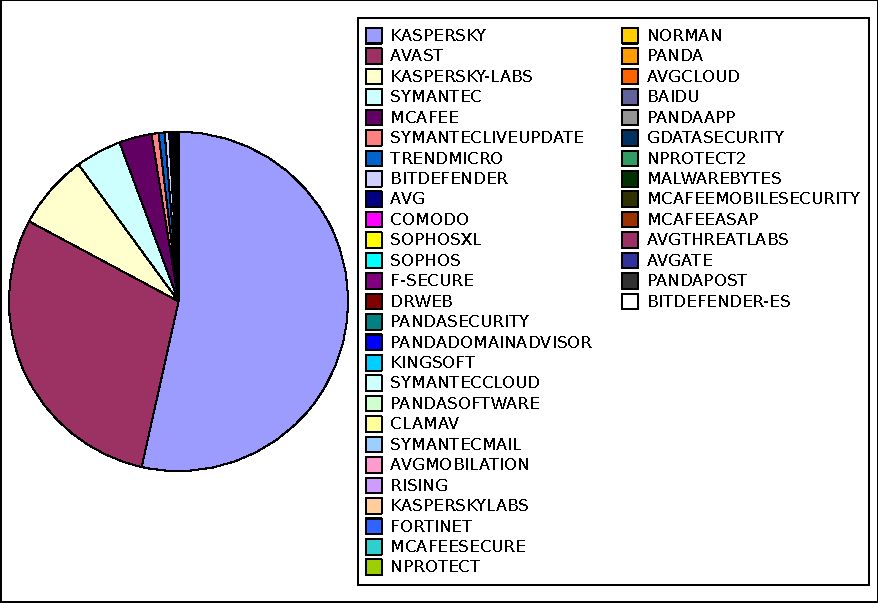
\includegraphics[scale=0.7]{av-stats.pdf}
\end{frame}


\begin{frame}
        {\center \it \Huge How do we collect all this crap?\\}
        \begin{flushright}
        by listening to the void
        \end{flushright}
\end{frame}


\begin{frame}
        \frametitle{Collection and Analysis Framework}
        \framesubtitle{Collection and Analysis Framework}
        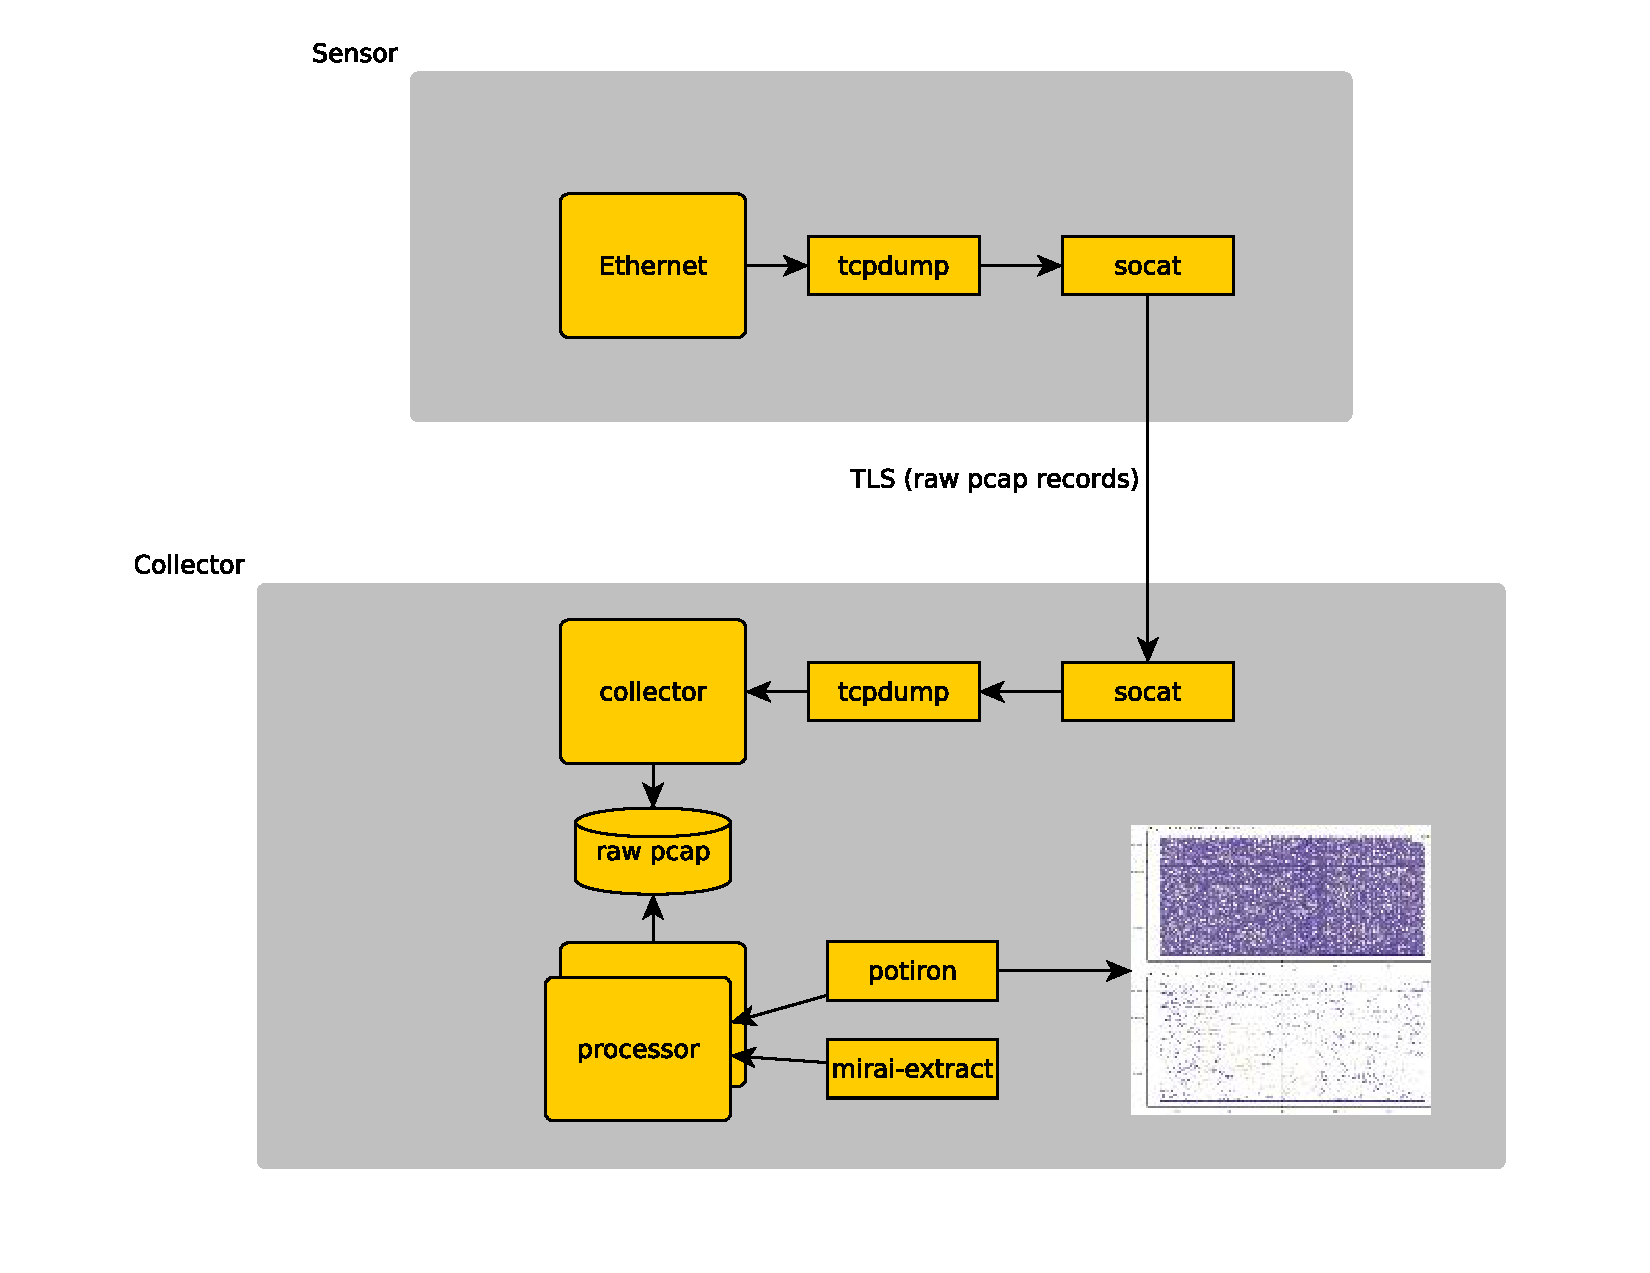
\includegraphics[scale=0.29]{overview-sensor.pdf}
\end{frame}


\begin{frame}
        \frametitle{Collection and Analysis Framework}
        \framesubtitle{or to keep the collection as simple as possible}
        \begin{itemize}
           \item Minimal sensor collecting IP-Darkspace networks (\textbf{close to RFC1918 address space})
           \item Raw pcap are captured with the full payload
           \item Netbeacon\footnote{\url{https://github.com/adulau/netbeacon/}} developed to ensure consistent packet capture
           \item Potiron\footnote{\url{https://github.com/CIRCL/potiron}} to normalize, index, enrich and visualize packet capture
        \end{itemize}
\end{frame}

\begin{frame}
        \frametitle{Blackhole \& honeypot operation}
        \framesubtitle{Collection and analysis framework}
        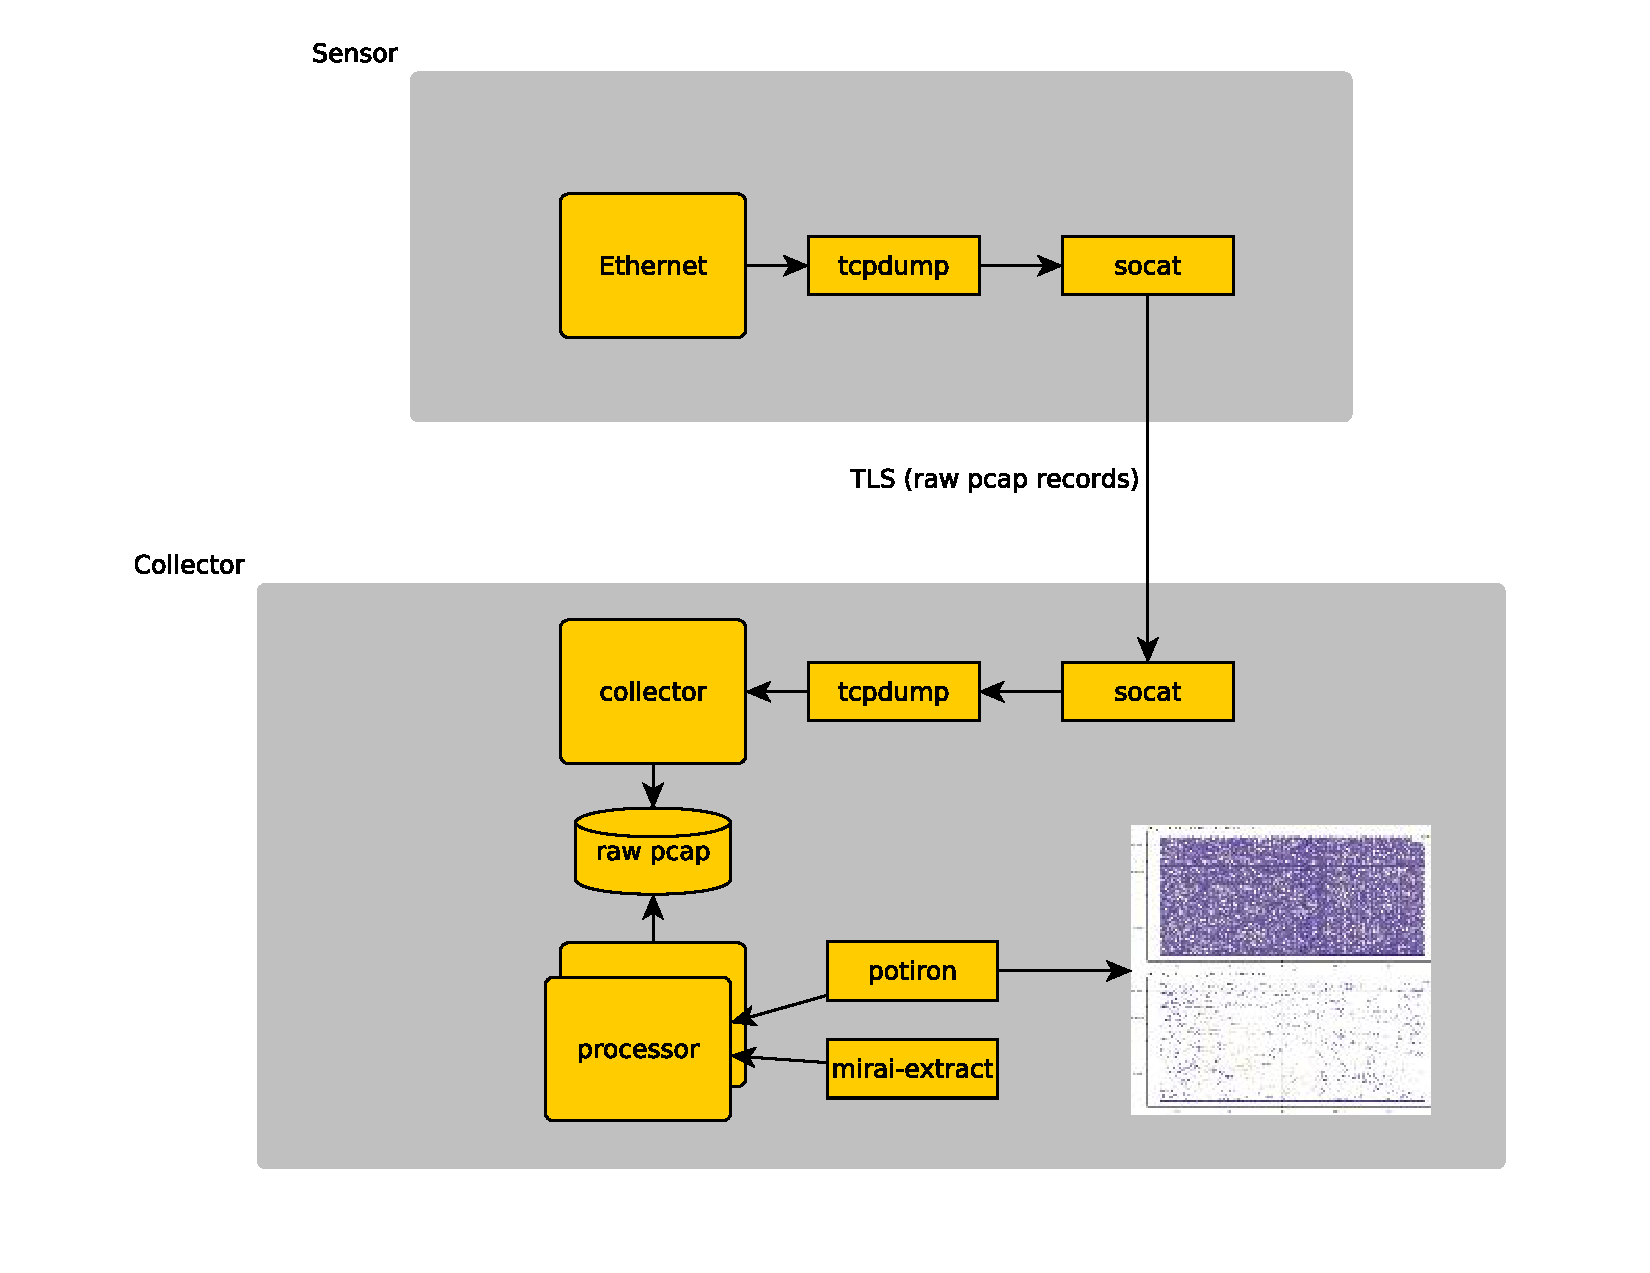
\includegraphics[scale=0.29]{overview-sensor.pdf}
\end{frame}

\begin{frame}
\frametitle{Blackhole operation}
    \begin{definition}[Principle]
        \begin{itemize}
            \item KISS (Keep it simple stupid)
            \item Linux \& OpenBSD operating systems
        \end{itemize}
    \end{definition}

    \begin{block}{Sensor}
    \lstset{%
        language=bash,
        backgroundcolor=\color{gray!25},
        basicstyle=\ttfamily,
        breaklines=true,
        columns=fullflexible
    }
    \begin{lstlisting}
tcpdump -l -s 65535 -n -i vr0 -w - '( not port $PORT and not host $HOST )' | socat - OPENSSL-CONNECT:$COLLECTOR:$PORT,cert=/etc/openssl/client.pem,cafile=/etc/openssl/ca.crt,verify=1
\end{lstlisting}


    \end{block}
\end{frame}


\begin{frame}
\frametitle{Dataset collected and statistics on one single blackhole}
\begin{itemize}
    \item From 2012-03-12 until Today (still active)
    \item More than 700 gigabytes of compressed raw pcap collected
    \item Constant stream of packets from two /22 network blocks
    \begin{itemize}
        \item no day/night profile.
    \end{itemize}
    \item Some peaks at 800kbit/s (e.g. often TCP RST from backscatter traffic but also from typographic errors)
\end{itemize}
\end{frame}



\begin{frame}
\frametitle{General observations}
\begin{itemize}
    \item A large part of traffic is coming from badly configured devices (\textbf{RFC1918 spelling errors})
    \begin{itemize}
        \item Printers, embedded devices, routers or even server.
        \item Trying to do name resolution on non-existing DNS servers, NTP or sending syslog messages.
    \end{itemize}
    \item Even if the black hole is passive, payload of stateless UDP packets or even TCP (due to asymmetric routing on misspelled network) datagrams are present
    \item Internal network scanning and reconnaissance tool (e.g. internal network enumerationi)
    \item The recursive effect of statistics (e.g. nmap-services)
\end{itemize}
\end{frame}


\begin{frame}
\frametitle{Observation per AS}
\framesubtitle{Traffic seen in the darknet}

\begin{columns}[b]
   \column{4cm}
        \begin{tabular}{lll}
        N&Frequency& ASN\\
        1 & 4596319 &4134\\
        2 &1382960 &4837\\
        3 &367515 &3462\\
        4 &312984 &4766\\
        5 &211468 &4812\\
        6 &166110 &9394\\
        7 &156303 &9121\\
        8 &153585 &4808\\
        9 &135811 &9318\\
        10 &116105 &4788\\
        \end{tabular}
   \column{6.4cm}
   \begin{block}{}
   \begin{itemize}
   \item Occurrences of activities related to the proportion of hosts in a country
   \item The Great Firewall of China is {\bf not filtering leaked packets}
   \item Corporate AS number versus ISP/Telco AS number
   \end{itemize}
   \end{block}
 \end{columns}

\end{frame}

\begin{frame}
        {\center \it \Huge How to build your "next" network reconnaissance tools?\\}
        \begin{flushright}
        by listening to the void
        \end{flushright}
\end{frame}



\begin{frame}[fragile]
\frametitle{Network reconnaissance (and potential misuse): DNS}
\lstset{ %
%language=Python,                % choose the language of the code
basicstyle=\footnotesize,       % the size of the fonts that are used for the code
numbers=left,                   % where to put the line-numbers
numberstyle=\footnotesize\color{cyan},      % the size of the fonts that are used for the line-numbers
stepnumber=1,                   % the step between two line-numbers. If it is 1 each line will be numbered
numbersep=5pt,                  % how far the line-numbers are from the code
backgroundcolor=\color{white},  % choose the background color. You must add \usepackage{color}
showspaces=false,               % show spaces adding particular underscores
showstringspaces=false,         % underline spaces within strings
showtabs=false,                 % show tabs within strings adding particular underscores
rulecolor=\color{red},
frame=single,           % adds a frame around the code
tabsize=2,          % sets default tabsize to 2 spaces
captionpos=b,           % sets the caption-position to bottom
breaklines=true,        % sets automatic line breaking
breakatwhitespace=false,    % sets if automatic breaks should only happen at whitespace
escapeinside={\%*}{*)}          % if you want to add a comment within your code
}

\begin{lstlisting}
3684 _msdcs.<companyname>.local
1232666 time.euro.apple.com
104 time.euro.apple.com.<mylocaldomain>
122 ocsp.tcs.terena.org
50000+ ocsp.<variousCA>
\end{lstlisting}
\begin{itemize}
\item DNS queries to an incorrect nameserver could lead to major misuse
\item {\bf A single typographic error in a list of 3 nameservers is usually unnoticed}
\end{itemize}
\end{frame}

\begin{frame}
\frametitle{Software Updates/Queries from Misconfigured Resolvers}
\begin{itemize}
\item Discovering software usage (and vulnerabilities) can be easily done with passive reconnaissance
\item Are the software update process ensuring the integrity of the updates?
\end{itemize}
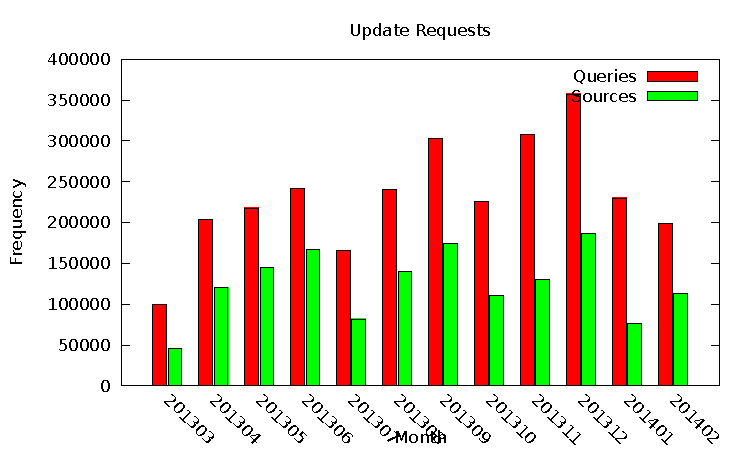
\includegraphics[scale=0.4]{update.pdf}
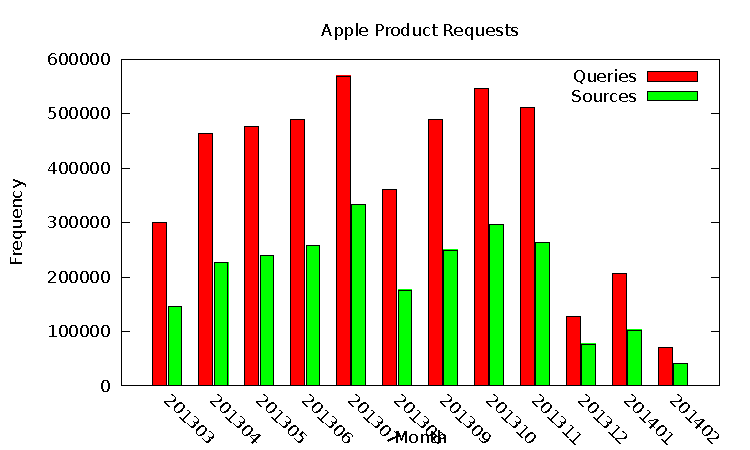
\includegraphics[scale=0.4]{apple.pdf}
\end{frame}


\begin{frame}
\frametitle{Network Reconnaissance - A source for your smart DNS Brute-Forcer}
\begin{tabular}{ll}
ASTTF.NET & HELP.163.COM\\
ASUEGYI.INFO & HP\_CLIENT1\\
ASUS1025C& MACBOOKAIR-CAD7\\
DEFAULT& MACBOOK-B5BA66\\
DELICIOUS.COM& MACBOOKPRO-5357\\
DELL& MAIL.AFT20.COM\\
DELL1400& S3.QHIMG.COM\\
DELL335873&SERVERWEB\\
DELL7777&SERVEUR\\
DELL-PC&SERVICE.QQ.COM\\
DELLPOP3&SMTP.163.COM\\
\end{tabular}
And many more ...
\end{frame}

\begin{frame}
        \frametitle{Building your DNS brute-forcer}
\begin{itemize}
        \item Smart DNS Brute-Forcer\footnote{\url{https://www.foo.be/papers/sdbf.pdf}}\footnote{\url{https://github.com/jfrancois/SDBF}} uses techniques from natural language modeling with Markov Chain Models
\item The processor relies on passive DNS data to generate the statistics and extract the features.
\item The DNS queries seen in the {\bf IP darkspace can be considered as a passive DNS stream} with a focus on internal network.
\item Providing a unique way to create {\bf internal DNS brute-forcers from external observations}.
\end{itemize}
\end{frame}

\begin{frame}
\frametitle{Network Reconnaissance: NetBios Machine Types (1 week)}
\begin{tabular}{ll}
     23 &Browser Server\\
      4 &Client$?$\\
      1 &Client$?$ M $<$ACTIVE$>$ \\
     21 &Domain Controller\\
      1 &Domain Controller M $<$ACTIVE$>$ \\
     11 &Master Browser\\
      1 &NameType=0x00 Workstation\\
      1 &NameType=0x20 Server\\
    105 &Server\\
     26 &Unknown\\
      1 &Unknown $<$GROUP$>$ B $<$ACTIVE$>$\\
      5 &Unknown $<$GROUP$>$ M $<$ACTIVE$>$\\
   1322 &Workstation\\
      1 &Workstation M $<$ACTIVE$>$ \\
\end{tabular}
\end{frame}


\begin{frame}[fragile]
\frametitle{How to configure your router (without security)}
\framesubtitle{Enable command logging and send the logs to a random syslog server}
\begin{verbatim}
Aug 13 10:11:51 M6000-G5 command-log:[10:11:51 08-13-2012
  VtyNo: vty1  UserName: XXX IP: XXX ReturnCode: 1
  CMDLine: show subscriber interface gei-0/2/1/12.60
Aug 13 10:46:05 M6000-G5 command-log:[10:46:05 08-13-2012
  VtyNo: vty2  UserName: XXX IP: XXX  ReturnCode: 1
  CMDLine: conf t ]
Aug 13 10:46:10 M6000-G5 command-log:[10:46:10 08-13-2012
  VtyNo: vty2  UserName: XXX IP: XXX  ReturnCode: 1  CMD
Line: aaa-authentication-template 1100 ]
...
\end{verbatim}
We will let you guess the sensitive part afterwards...
\end{frame}

\begin{frame}
\frametitle{Finding origin of traffic by TCP sequence analysis}
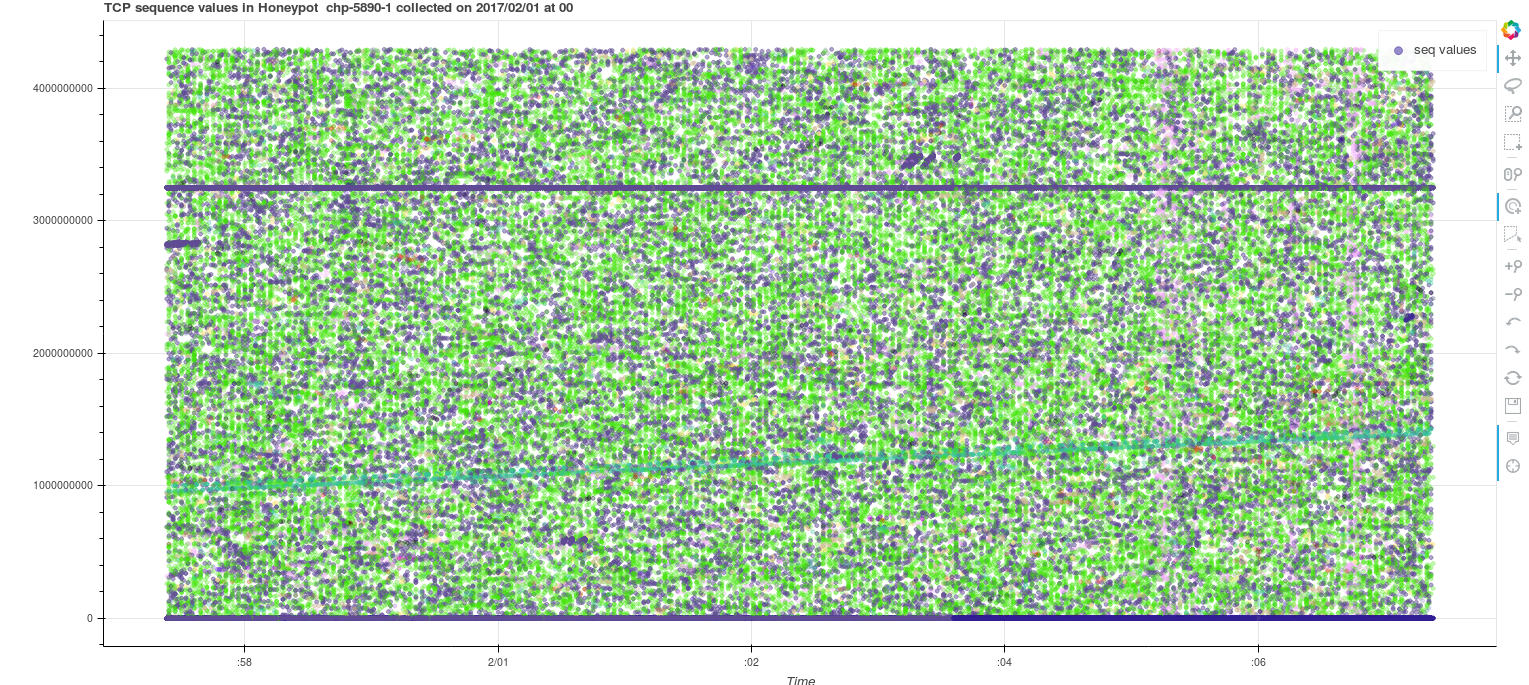
\includegraphics[scale=0.21]{isn-1.png}
\end{frame}

\begin{frame}
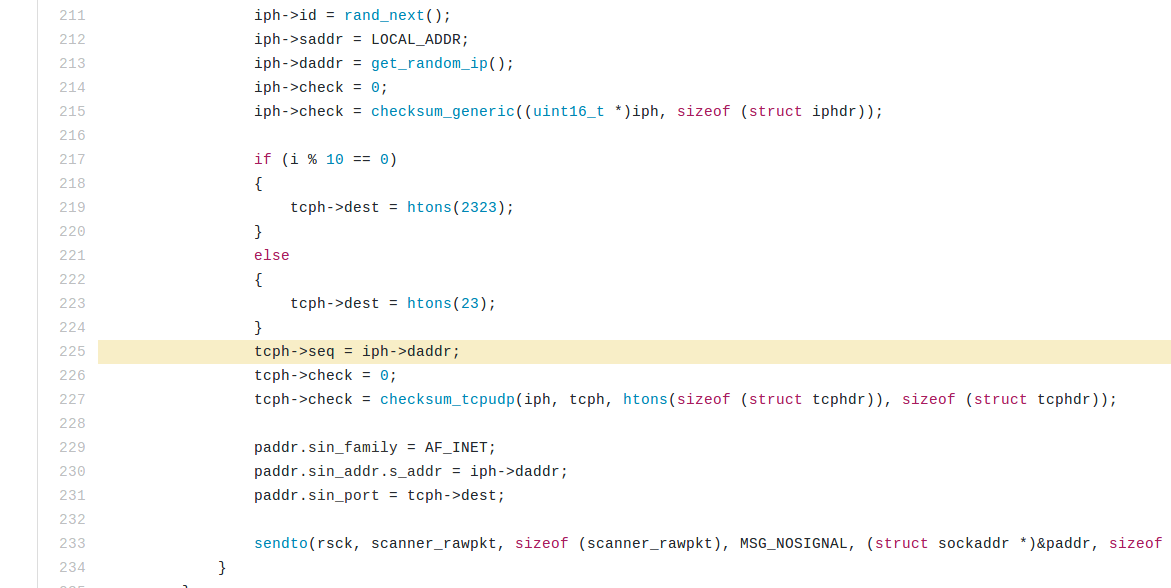
\includegraphics[scale=0.21]{mirai-isn.png}
\end{frame}

\begin{frame}
        \frametitle{Recommendations for operating an IP darkspace}
        \begin{itemize}
                \item {\bf Capture raw packets at the closest point}, don't filter, don't try to be clever, just store it as it.
                \item {\bf Test your network collection mechanisms} and storage. Send test network beacons. Check the integrity, order and completness of packets received.
                \item You never know in advance which features is required to distinguish a specific pattern.
                \item Did I mention to store {\bf RAW PACKETS}?
        \end{itemize}
\end{frame}

\begin{frame}
        \frametitle{Security conclusions}
\begin{itemize}
   \item Security recommendations
\begin{itemize}
    \item \textbf{Default routing/NAT to Internet in operational network is evil}
    \item Use fully qualified domain names (resolver search list is evil too)
    \item Double check syslog exports via UDP (e.g. information leakage is easy)
    \item Verify any default configuration with SNMP (e.g. enable by default on some embedded devices)
\end{itemize}
   \item Offensive usage? What does it happen if a malicious "ISP" responds to misspelled RFC1918 addresses? (e.g. DNS/NTP requests, software update or proxy request)
   \item Some research projects on this topic? Contact us \url{mailto:info@circl.lu}
\end{itemize}
\end{frame}

\begin{frame}
        \frametitle{IP darkspace and LE conclusions}
        \begin{itemize}
                \item \textbf{IP darkspace can be a complementary source of intelligence}
                \item Many network telescope are operated by researchers and have different way to collect network packets and provide access
                \item CIRCL recently started the D4 project\footnote{\url{https://www.d4-project.org/}}, to provide an unified way to collect network packets from distributed IP darkspaces and provide unified access to contributors
                \item Some IP darkspace are more interesting than others depending of the case investigated (e.g. DDoS tooling always spoofing specific network spaces, networks addresses similar to RFC1918)
        \end{itemize}

\end{frame}

\end{document}

